\chapter{Le Machine Learning}

Dans le cadre du rapport de stage, je vais me focaliser sur l'approche \textit{représentation et raisonnement}.\\
\linebreak
Un \textit{Dataset} est un tableau représentant pour chaque colonnes une donnée et pour chaque ligne un \textit{sample}, les samples sont composé d'une et d'une seul valeur par colonne, cette valeur peut être n'importe quoi (chaine de caractère, tableau, entier, boolean, ...). Un des format les plus utilisé pour illustrer la table est le format \textit{csv}, \textit{SQL} ou \textit{excel}.\\
\pagebreak

\section{Les premiers pas}

Dans les années 1950, on ne parlait pas encore du \textit{Machine Learning} que l'on n'a maintenant, on parlait de méthode de généralisation d'un modèle.\\
Imaginons que vous vouliez prédire un résultat de type boolean à partir de données que vous avez enregistré.

\begin{center}
\begin{multicols}{3}
[Sans tout ses algorithmes de machines learning actuel, le principe était de généraliser le modèle au maximum,pour ceci avec un trahit puis pour chaque ligne faire l'intersection avec le trahit, tout ceci donne $\crouge{c}$:]

\begin{tabular}{ccc|c}
A & B & C & résultat \\
\hline
0 & 0 & 1 & 1\\
0 & 1 & 1 & 1\\
1 & 1 & 0 & 0\\
\end{tabular}
\scalebox{0.4}{
\begin{tikzpicture}[->,>=stealth',shorten >=1pt,auto,node distance=2.8cm,
                    semithick]
  \tikzstyle{every state}=[fill=white,draw=none,text=black]

  \node[state]         (Z)                    {$\{\}$};
  \node[state]         (B) [below  of=Z]      {$B$};
  \node[state]         (A) [left  of=B]       {$A$};
  \node[state]         (C) [right of=B]       {$\crouge{C}$};
  \node[state]		   (AB) [below of=A]      {$AB$};
  \node[state]		   (AC) [right of=AB]     {$AC$};
  \node[state]         (BC) [right of=AC]     {$BC$};
  \node[state] 		   (ABC) [below of=AC]    {$ABC$};
  

  \path (Z) edge              node {} (A)
            edge              node {} (B)
            edge			  node {} (C)
        (A) edge			  node {} (AB)
        	edge			  node {} (AC)
        (B) edge			  node {} (AB)
        	edge			  node {} (BC)
        (C) edge 			  node {} (AC)
        	edge			  node {} (BC)
        (AB) edge 			  node {} (ABC)
        (AC) edge			  node {} (ABC)
        (BC) edge			  node {} (ABC);
\end{tikzpicture} }
\end{multicols}
\end{center}

Cette technique, beaucoup utilisé en fouille de données, a ses limites, quelques années plus tard vient les premiers algorithmes de machine learning qui de nos jours sont encore bien répandue, en voici une liste non exhaustif:

\begin{description}
\item[Gradient]: Pour un nuage de points, le but est de trouver une droite qui minimise la distance (sur l'axe Y) entre celle ci et chaque  points du nuage.
\item[Kmeans]: Pour chaque sample du dataset, le but est de former des groupes de samples qui se ressemble le plus.
\end{description}

Ci dessus, deux modèle du machines learning, le Gradient est un modèle dit \textit{Supervisé} et le Kmeans est dit \textit{Non Supervisé}. La différence entre les deux modèle et simple, soit un dataset possédant une colonne nommé \textit{Étiquette} (ou Class en anglais) donne le résultat du sample concerné, il est donc facile pour un sample possédant une colonne Étiquette de connaitre son appartenance, on dit alors que le modèle est supervisé, pour un modèle non supervisé, nous ne connaissons pas les étiquettes des samples.\\
\pagebreak

\section{Algorithmes d'apprentissage}

De nos jours il existe une tonne d'algorithme d'apprentissage, tout ont plus ou moins leurs utilité, avantage, faiblesse, d'où le fait que pour le data scientiste doit essayer un peu tout les algorithmes et de juger de leurs efficacité via les résultats donnée. Bien-sûr si un Gradient suffit pourquoi vouloir utiliser un réseaux de neurones.\\
En voici une liste non exhaustive utilisé lors du stage à des fins de teste (via la librairie sci-kit-learn de python):

\begin{description}
\item[Support Vector Machine]: Le support vector machines cherche un hyperplan (de couleur noir) pouvant départager des classes,
Il en existe une infinité d'hyperplan qui peuvent les départager, donc introduisons un autre concept, celui de 
l'hyperplan qui maximise la séparation entre les deux classes (les droites $\corange{Oranges}$ appelé $Margin$.\\
\cshape{0.5}{
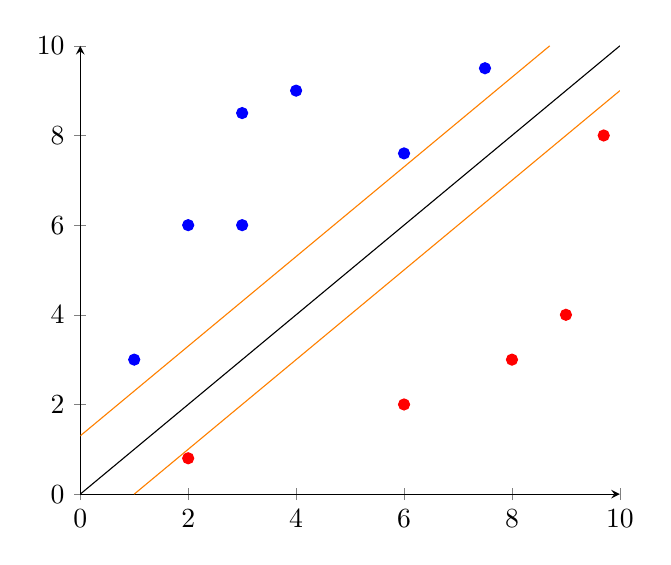
\begin{tikzpicture}
  \begin{axis} [
      axis lines = left,
      xmin       = 0,
      ymin       = 0,
    ]
    \addplot [color=black] coordinates {(0,0)(10,10)};
    \addplot [color=orange] coordinates {(0,1.3)(8.7,10) };
    \addplot [color=orange] coordinates {(1,0)(10,9) };
    \addplot [only marks, mark=*, color=blue] coordinates {(2,6)(1,3)(6,7.6)(3,8.5)(7.5,9.5)(4,9)(3,6)};
    \addplot [only marks, mark=*, color=red]  coordinates {(2,0.8)(6,2)(9,4)(9.7,8)(8,3)};
  \end{axis}
\end{tikzpicture}
}

\item[Decision Tree]: Un arbre de décision est une suite de nœuds relié par au moins une arrête, on emprunte une arrête par rapport à la décision qui est à prendre via le nœuds courant. L'ordre des nœuds est choisis selon des critères (les trois les plus utilisé sont \textit{Entropy}, \textit{Information grain} et \textit{Gini}), ces trois critères de sélection appliqué au même dataset peut donner un arbre diffèrent. Une feuille d'arbre est un nœuds n'ayant aucun fils, les étiquettes des prédictions s'y trouve.
\cshape{0.5}{
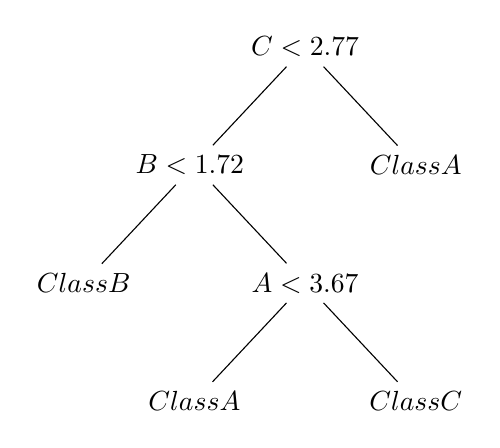
\begin{tikzpicture}[sibling distance=8em,
  every node/.style = {scale=1,
    draw=none, align=center}]]
  \node {$C < 2.77$}
 	  child { node {$B < 1.72$ }
 	    child { node {$Class B$}}
 	    child { node {$A < 3.67$}
 	      child { node {$Class A$}
 	      }
 	      child { node {$Class C$} }
 	    }
 	  }
 	  child { node {$Class A$} }
    ;
\end{tikzpicture}
}
\end{description}

\pagebreak
Traiter les samples de type numérique donne beaucoup de possibilités de traiter un problème.\\
L'évolution a fait que de plus de données sont de type textuel, pour des dates et durées, le problème reste simple à résoudre, pour une suite de mots fini, il suffit de les énumérer, mais pour les données du langage naturel?\\
\linebreak

\section{Langage naturel}

Un texte peu être long ou court, contenant des liens, des caractères spéciaux, on ne peut pas utiliser lancer un algorithme comme ci dessus sur des textes et en espérer en tirer de bon résultats, plusieurs étapes sont nécessaire pour pouvoir utiliser des algorithmes qui travaillent avec des textes. 

\subsection{Nettoyage des données}

Le français est un langage riche en dérivé de lettres notamment pour ses caractères accentués, le premier travail est de réduire l'espace des caractères en éliminent par exemple les majuscules et les remplacer par des minuscules, éliminer la ponctuation, puis normaliser les accents. Nous pouvons obtenir un texte comme suite:
\\
\sepline\\
Bonjour, je viens parce-que j'ai une fuite d'eau sur mon plafond, j'ai déjà prit contact avec une entreprise pour ses réparations mais elle n'a pas donné suite.\\
\sepline\\
bonjour je viens parce que j ai une fuite d eau sur mon plafond, j ai deja prit contact avec une entreprise pour ses reparations mais elle n a pas donne suite\\
\sepline\\

